\documentclass{handout}

% \SetInstructor{Lt Col James Phillips}
\SetCourseTitle{ECE231: Electrical Circuits and Systems I}
\SetSemester{Fall 2016}
\SetHandoutTitle{Lecture 13: Circuits with Dependent Sources}
%\SetDueDate{1 Jan 2016}
%\ShowAllBlanks

\showsoln \setsolncolor{red}

\begin{document}
\maketitle

\textbf{OBJECTIVES:}
\begin{enumerate}
\item Understand and Analyze circuits with dependent sources
\end{enumerate}

\textbf{READING}
\begin{description}
\item [Required]:
\begin{itemize}
\item  Textbook, sections 4.1--4.2
\end{itemize}
\item [Optional]: None
\end{description}

\section{Preliminary Definitions}

\begin{description}
	\item[Active device] -- Any component that requires an external power supply to operate correctly. {\em Any device that has a gain greater than 1 is an active device}
	\item[Active circuit] -- Any circuit with at least one active device
	\item[Gain] -- The ratio of our output signal to our input signal (assumes input and output have the same dimensions)
	\item[Signal ampliflication] -- A gain greater than 1
	\item[Dependent source] -- A voltage or current source whose output is controlled by a voltage or current elsewhere in the circuit
\end{description}

\section{Types of dependent sources}
Since dependent sources can supply voltage or current and they are controlled by voltage or current elsewhere, we can have 4 types of dependent sources:

\soln{3in}{
\begin{enumerate}
	\item Voltage Controlled Voltage Source (VCVS)
	\item Current Controlled Voltage Source (CCVS)
	\item Voltage Controlled Current Source (VCCS)
	\item Current Controlled Current Source (CCCS)
\end{enumerate}
}

\newpage
\clearpage
\pagebreak

\begin{figure} [h! t! b!]
\centering
\soln{2.5in}{
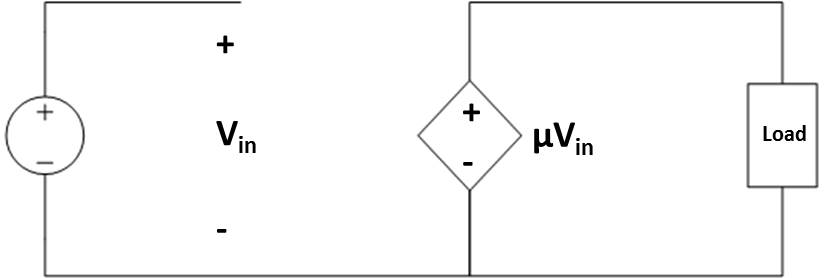
\includegraphics[width=0.5\textwidth]{VCVS.jpg}
}
\caption{Voltage Controlled Voltage Source, note, the diamond shaped source is
the depended one}
\label{fig: VCVS}
\end{figure}

\begin{figure} [h! t! b!]
\centering
\soln{2.5in}{
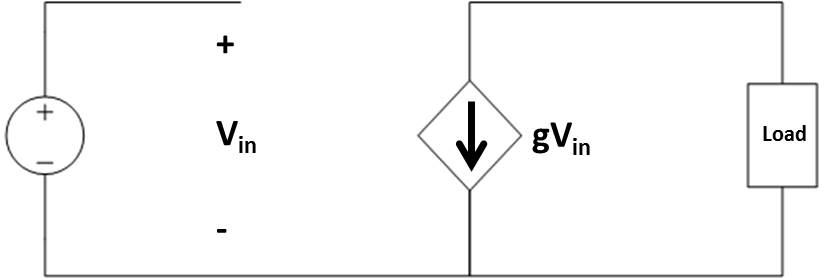
\includegraphics[width=0.5\textwidth]{VCCS.jpg}
}
\caption{Voltage Controlled Current Source}
\label{fig: VCCS}
\end{figure}

\begin{figure} [h! t! b!]
\centering
\soln{2.5in}{
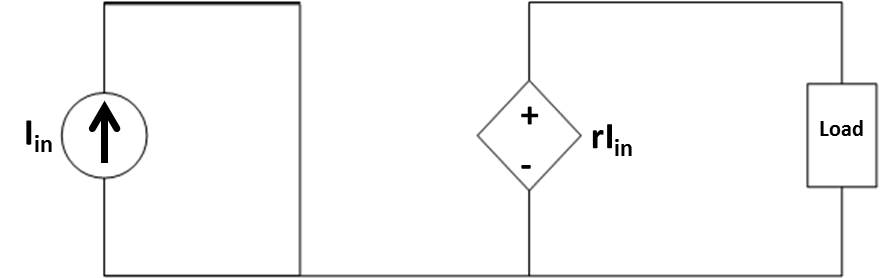
\includegraphics[width=0.5\textwidth]{CCVS.jpg}
}
\caption{Current Controlled Voltage Source}
\label{fig: CCVS}
\end{figure}

\begin{figure} [h! t! b!]
\centering
\soln{2.5in}{
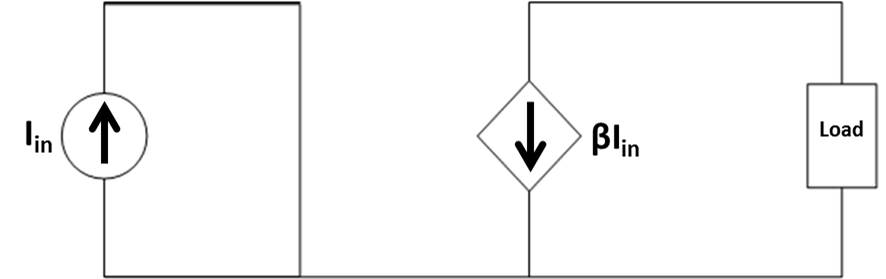
\includegraphics[width=0.5\textwidth]{CCCS.jpg}
}
\caption{Current Controlled Current Source}
\label{fig: CCCS}
\end{figure}

Figures \ref{fig: VCVS} -- \ref{fig: CCCS} show all the possible dependent
source arrangements. It is worth noting that the control signal does not have
to be an independent source, but rather can be any current or voltage in the
circuit.

\soln{1in}{
% In Figure \ref{fig: VCVS}, $\mu$ is the voltage gain and is unitless.
%
% In Figure \ref{fig: VCCS}, $g$ is the transconductance and has the units of Siemens.
%
% In Figure \ref{fig: CCVS}, $r$ is the transresistance and has the units of Ohms.
%
% In Figure \ref{fig: VCVS}, $\beta$ is the current gain and is unitless.

	\begin{table}[!h]
		\centering
		\begin{tabular}{|l|c|c|c|l|}
			\hline
			Source & In & Out & Gain & Units \\
			\hline
			VCVS & V & V & $\mu$ & unitless \\
			VCCS & V & I & $\gamma$ & Siemens \\
			CCVS & I & V & $r$ & Ohms \\
			CCCS & I & I & $\beta$ & unitless \\
			\hline
		\end{tabular}
	\end{table}
}

\newpage
\clearpage
\pagebreak

\section{Circuit Analysis with Dependent Sources}
All circuit analysis techniques we have already learned work with Dependent sources with some caveats....
\soln{2in}{
\begin{enumerate}
\item Dependent sources cannot be turned off independent of the controlling current or voltage; that is to turn off a dependent source, you have to turn off the controlling current or voltage.  This is often not practical; therefore, superposition is not normally used for dependent sources
\item Circuit reduction and source transformation can be used, provided you do not eliminate the control variable
\end{enumerate}
}

\textbf{Example 1 -- Textbook Exercise 4-1}
For the circuit shown in Figure \ref{fig: Example1}, find $v_o$ in terms of $v_s$

% Use this example to illustrate that no current flows in the bottom connecting wire

\begin{figure} [h! t! b!]
\centering
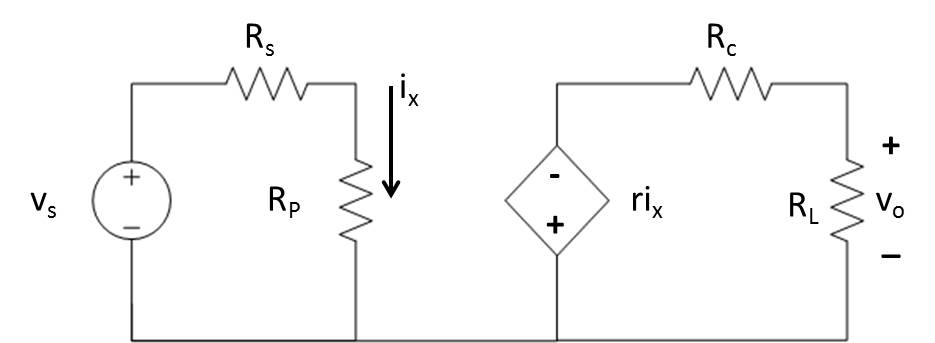
\includegraphics[width=0.5\textwidth]{Example1.jpg}
\caption{Circuit to accompany Example 1}
\label{fig: Example1}
\end{figure}
% \soln{6in}{
% \begin{figure}[h! t! b!]
% \centering
% 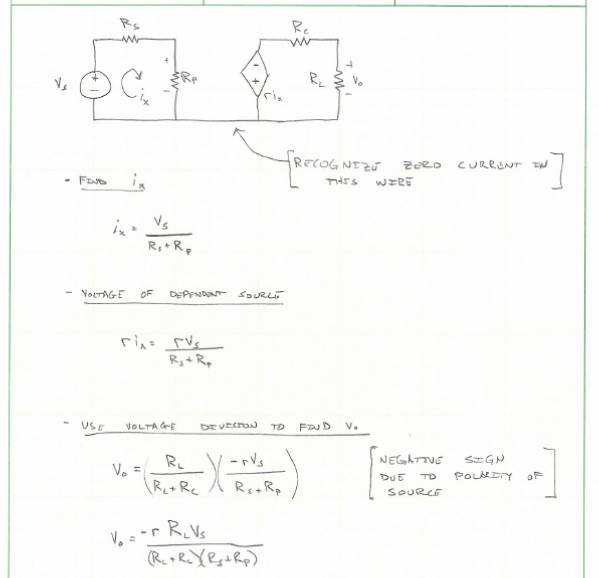
\includegraphics[width=0.7\textwidth]{Example1soln.jpg}
% \end{figure}
% }

\soln{\textwidth}{
	Note: there is zero current running through the single wire connecting the two loops together.
	\begin{eqnarray}
		i_x = \frac{V_s}{R_s + R_p} \\
		r i_x = \frac{r V_s}{R_s + R_p} \\
		V_o = \frac{R_L}{R_L + R_c} \frac{-r V_s}{R_s + R_p} & & \textsf{negative sign due to polarity of source} \\
		V_o = \frac{-r R_L V_s}{(R_L + R_c)(R_s + R_p)} \\
	\end{eqnarray}
}


\newpage
\clearpage
\pagebreak

\textbf{Example 2}
For the circuit shown in Figure \ref{fig: Example2}, find $v_o$ in terms of $v_s$

\begin{figure}[h! t! b!]
\centering
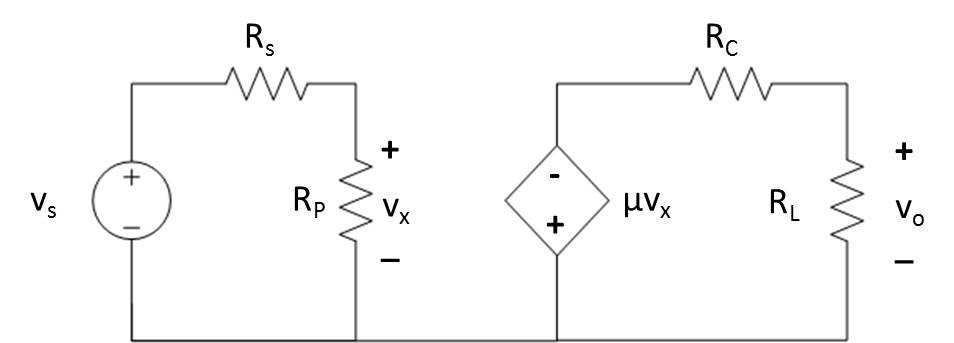
\includegraphics[width=0.5\textwidth]{Example2.jpg}
\caption{Circuit to accompany Example 2}
\label{fig: Example2}
\end{figure}

% \soln{6in}{
% \begin{figure}[h! t! b!]
% \centering
% 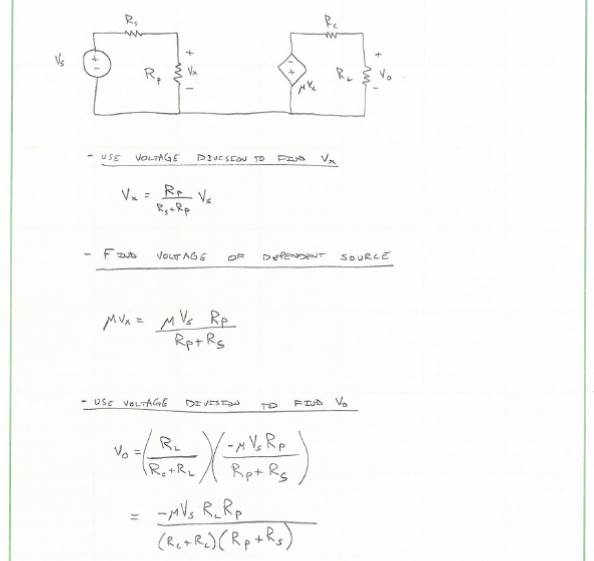
\includegraphics[width=0.8\textwidth]{Example2soln.jpg}
% \end{figure}
% }

\soln{\textwidth}{
	\begin{eqnarray}
		\textsf{voltage division:} & & V_x = \frac{R_p}{R_s + R_p} V_s \\
		\textsf{voltage of dependent source:} & & \mu V_x = \frac{R_p}{R_p + R_s} \mu V_s\\
		\textsf{voltage division to find} & V_o: \nonumber \\
		V_o = \frac{R_L}{R_L + R_c} \frac{-R_p}{R_s + R_p} \mu V_s \\
		V_o = \frac{-r V_s R_L R_p}{(R_L + R_c)(R_s + R_p)} \\
	\end{eqnarray}
}

\newpage
\clearpage
\pagebreak

\section{Nodal Analysis}
Recall the steps for writing node voltage equations:
\begin{enumerate}
	\item Identify a \textbf{reference node}.  You will not write an equation for this node, but the voltages at the other nodes will use this as a reference.
	\item Write \textbf{KCL equations} at the other $N-1$ nodes
	\item Write the currents in the KCL equations in terms of \textbf{node voltages} and resistances
	\item Rearrange the equations above into \textbf{standard form}
\end{enumerate}

Also recall that adding a voltage source to the circuit added additional constraints and we had three methods for dealing with those constraints
\begin{enumerate}
	\item Source transformation
	\item Smart choice of your reference node
	\item Define a {\em Supernode}
\end{enumerate}

All these methods still apply to circuits with dependent sources.  We will demonstrate by example:


%\textbf{Example 3} -- For the circuit shown in Figure \ref{fig: Example3},
%\begin{itemize}
%\item Write Node Voltage equations
%\item Write and expression for $v_o$ as a function of $R_F$
%\end{itemize}

%\begin{figure}[h! t! b!]
%\centering
%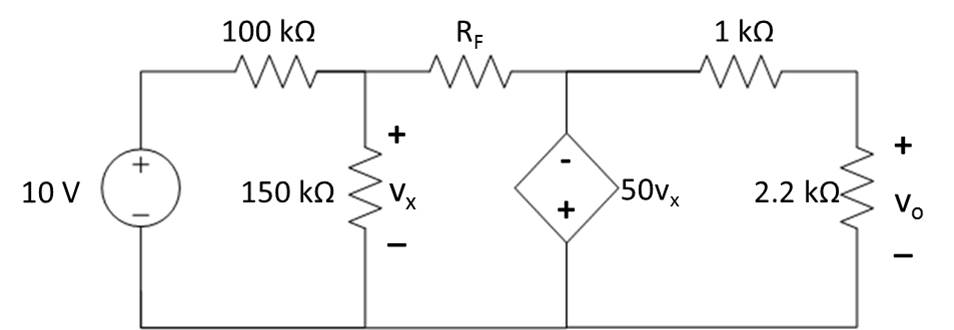
\includegraphics[width=0.5\textwidth]{Example3.jpg}
%\caption{Circuit to accompany Example 3}
%\label{fig: Example3}
%\end{figure}

% \soln{5in}{
% 	Step 1. Assign nodes (A-D across top)
%
% 	Stop 2. Write KCL eqns and constant equations
%
% 	\begin{eqnarray}
% 		V_A = 10 \\
% 		\frac{V_B - V_A}{100k} + \frac{V_B}{150k} + \frac{V_B - (-50)}{R_F} = 0 & & \because V_B = V_x \\
% 		V_c = -50 V_x = -50 V_B  \\
% 		\frac{V_o}{2.2k} + \frac{V_o - V_c}{1k} = 0 & & \because V_D = V_o  \\
% 	\end{eqnarray}
%
% 	Step 3. Now combine these eqns to get one composed of $V_o$ and $V_x$S
%
% 	\begin{eqnarray}
% 		\frac{V_x - 10}{100k} + \frac{V_x}{150k} + \frac{V_x - (-50 V_x)}{R_F} = 0 \\
% 		V_x \left( \frac{1}{100k} + \frac{V_x}{150k} + \frac{51}{R_F} \right) = \frac{10}{100k} \\
% 		\frac{V_o}{2.2k} + \frac{V_o -(-50 V_x)}{2.2k} = 0 \\
% 	\end{eqnarray}
%
% 	Step 4. Solve for $V_x$ in terms of $R_F$
%
% 	\begin{eqnarray}
% 		V_x = \frac{10}{100k} \left( \frac{1}{100k} + \frac{1}{150k} + \frac{1}{R_F} = \frac{10}{100k} \left( \frac{300k R_F}{5 R_F + 15.3M} \right) \\
% 		V_x = \frac{30 R_F}{5 R_F + 15.3 M} = \frac{6 R_F}{R_F + 3.06 k} \\
% 	\end{eqnarray}
% }

% \textbf{Example 3} -- For the circuit shown in Figure \ref{fig: Example3},
% \begin{itemize}
% \item Write Node Voltage equations
% \item Write and expression for $v_o$ as a function of $R_F$
% \end{itemize}
% \begin{figure}[h! t! b!]
% \centering
% 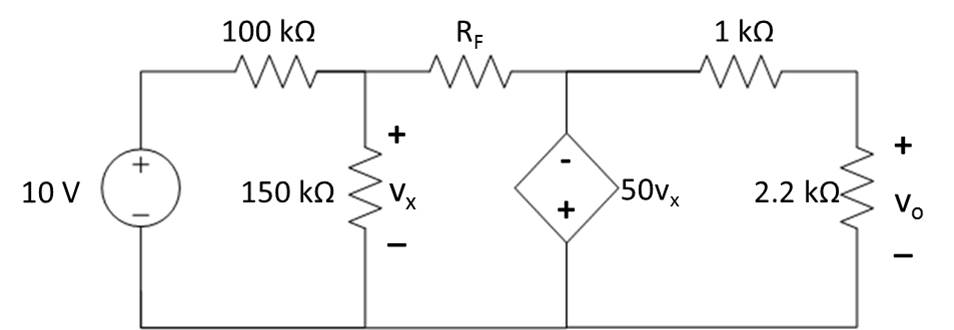
\includegraphics[width=0.5\textwidth]{Example3.jpg}
% \caption{Circuit to accompany Example 3}
% \label{fig: Example3}
% \end{figure}


\soln{18in}{
\begin{figure}[h! t! b!]
\centering
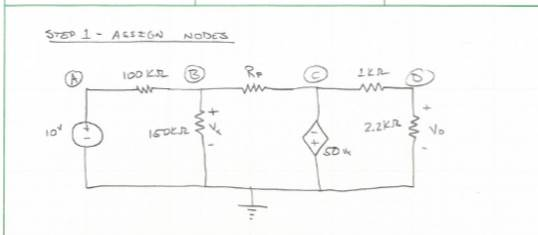
\includegraphics[width=0.7\textwidth]{Example3solnA.jpg}
\end{figure}

\newpage
\clearpage
\pagebreak

\begin{figure}[h! t! b!]
\centering
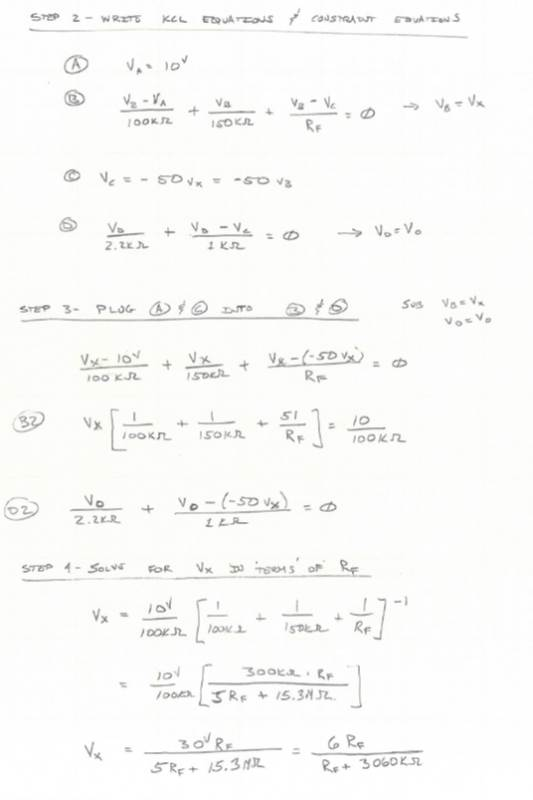
\includegraphics[width=0.9\textwidth]{Example3solnB.jpg}
\end{figure}

\newpage
\clearpage
\pagebreak

\begin{figure}[h! t! b!]
\centering
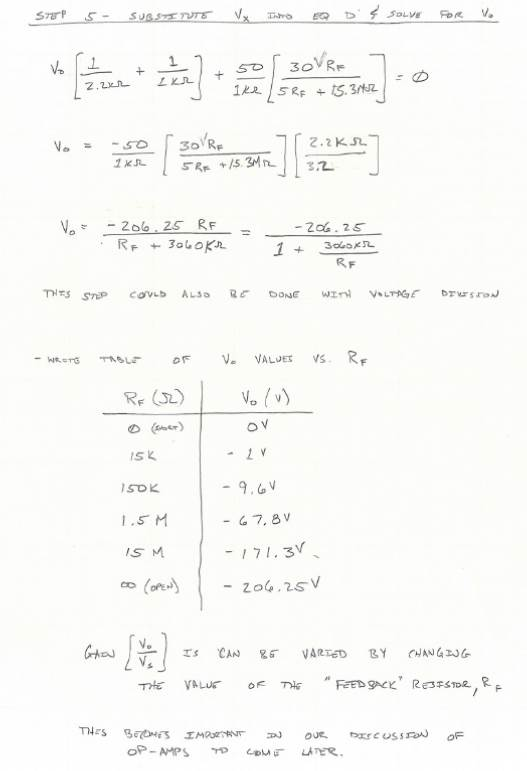
\includegraphics[width=0.9\textwidth]{Example3solnC.jpg}
\end{figure}

}
\newpage
\clearpage
\pagebreak

\textbf{Example 4 -- Textbook Exercise 4-2}
For the Circuit shown in Figure \ref{fig: Example4}, write an expression for the gain ($K=\frac{v_O}{v_S}$) in terms of $R_F$ then find values for $R_F$ such that $50<|K|<10,000$ (given that $\mu=10^5$).
\begin{figure}[h! t! b!]
\centering
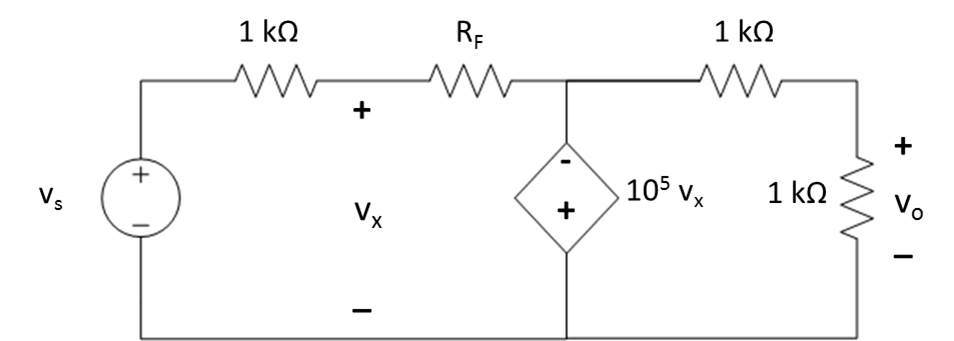
\includegraphics[width=0.6\textwidth]{Example4.jpg}
\caption{Circuit to accompany Example 4}
\label{fig: Example4}
\end{figure}

\soln{18in}{
\begin{figure}[h! t! b!]
\centering
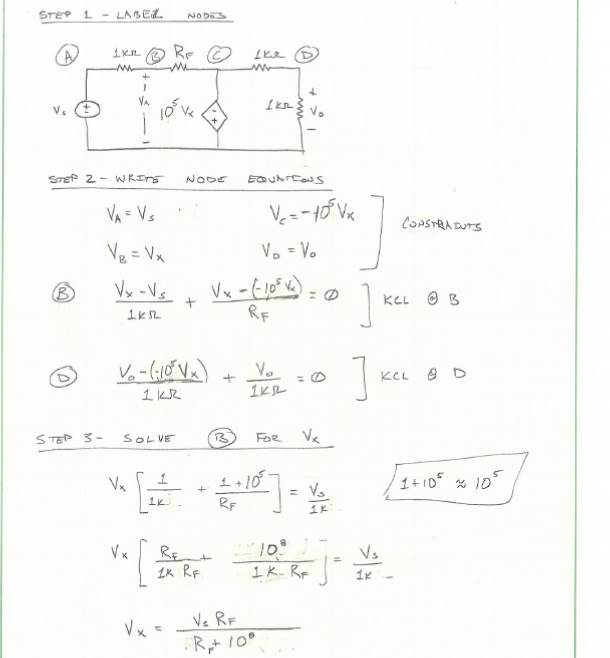
\includegraphics[width=0.8\textwidth]{Example4solnA.jpg}
\end{figure}

\newpage
\clearpage
\pagebreak

\begin{figure}[h! t! b!]
\centering
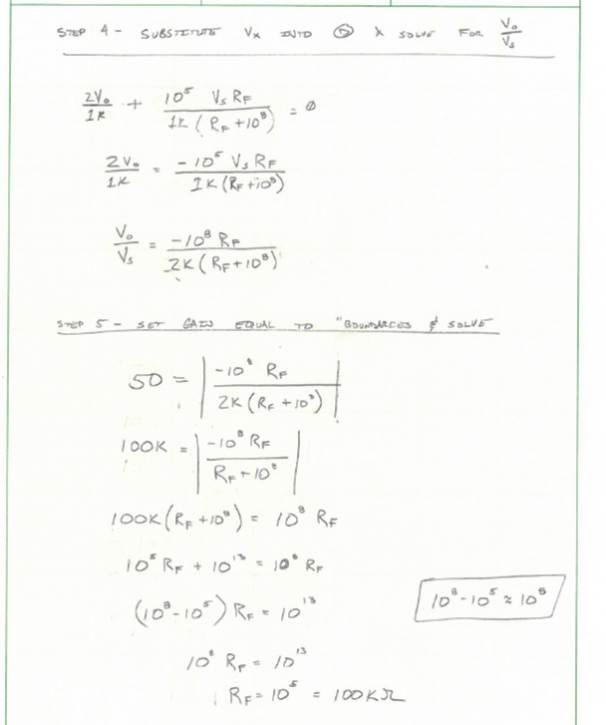
\includegraphics[width=0.9\textwidth]{Example4solnB.jpg}
\end{figure}

\newpage
\clearpage
\pagebreak

\begin{figure}[h! t! b!]
\centering
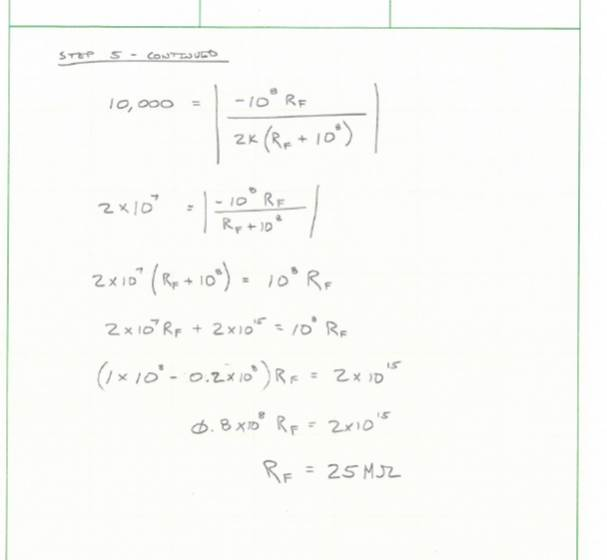
\includegraphics[width=0.9\textwidth]{Example4solnC.jpg}
\end{figure}

}

\newpage
\clearpage
\pagebreak

\section{Mesh Analysis}
Recall the steps for writing Mesh Current equations:
\begin{enumerate}
\item Assign a current to each mesh
\item Assign a voltage (magnitude and polarity) to each device in the circuit
\item Write Kirchhoff's Voltage Law (KVL) equations for each mesh
\item Use device $i$--$v$ characateristics to rewrite KVL eqations from the previous step
\item Rewrite equations in standard (matrix) form
\end{enumerate}

Futhermore, recall the 3 methods for dealing with current sources
\begin{enumerate}
\item Use source transformation to eliminate current sources
\item When possible assign meshes so the source is only part of one mesh
\item Use a {\em Supermesh}
\end{enumerate}

All these methods can be used when dealing with cicuits with dependent sources.  We will demonstrate with examples:

\newpage
\clearpage
\pagebreak

\textbf{Example 5 -- Textbook Exercise 4-8}
Use mesh analysis to find the current $i_O$ in Figure \ref{fig: Example5}.
\begin{figure}[h! t! b!]
\centering
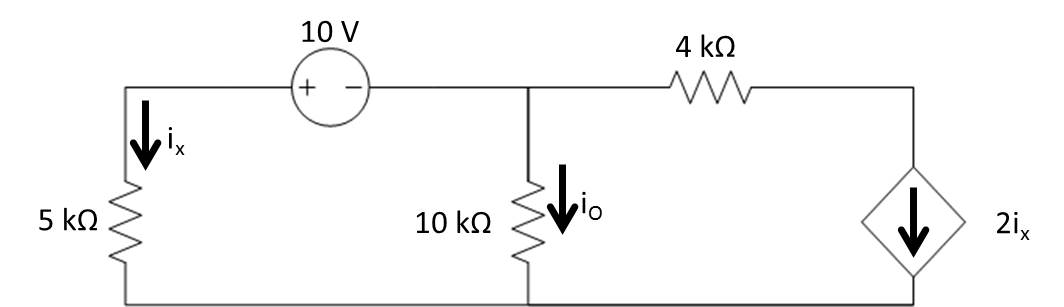
\includegraphics[width=0.6\textwidth]{Example5.jpg}
\caption{Circuit to accompany Example 5}
\label{fig: Example5}
\end{figure}

\soln{6in}{
\begin{figure}[h! t! b!]
\centering
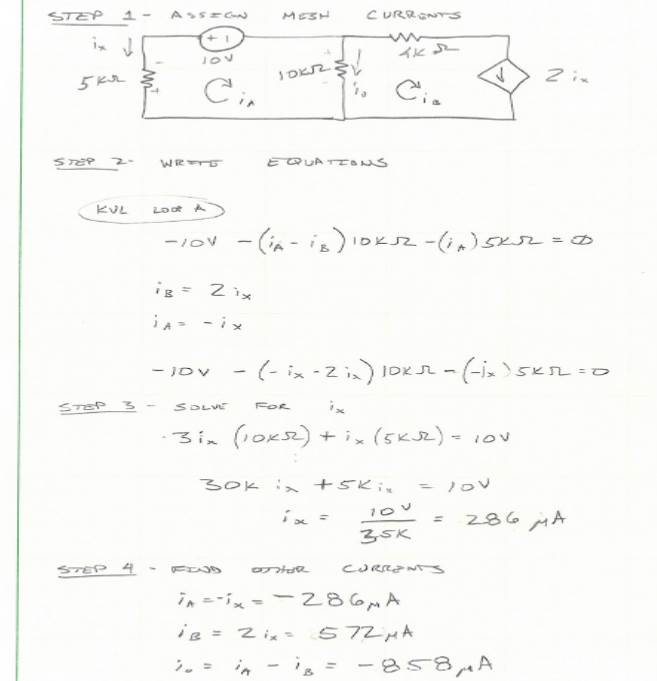
\includegraphics[width=0.6\textwidth]{Example5soln.jpg}
\end{figure}
}

\newpage
\clearpage
\pagebreak

\textbf{Example 6 -- Textbook Exercise 4-9}
Use mesh analysis to find the current $i_O$ in Figure \ref{fig: Example6}.
\begin{figure}[h! t! b!]
\centering
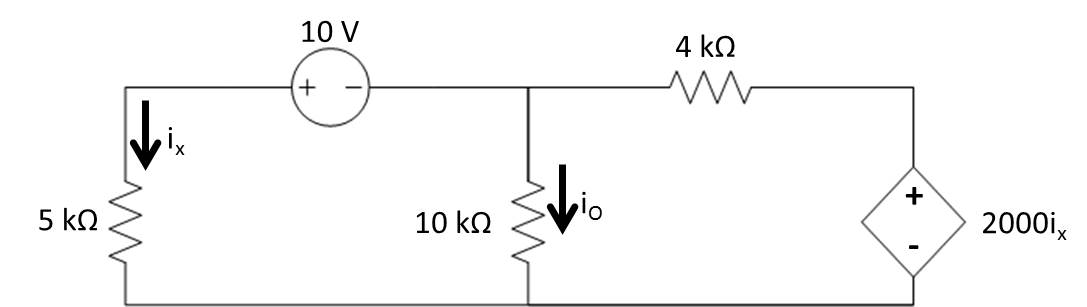
\includegraphics[width=0.6\textwidth]{Example6.jpg}
\caption{Circuit to accompany Example 6}
\label{fig: Example6}
\end{figure}

\soln{6in}{
\begin{figure}[h! t! b!]
\centering
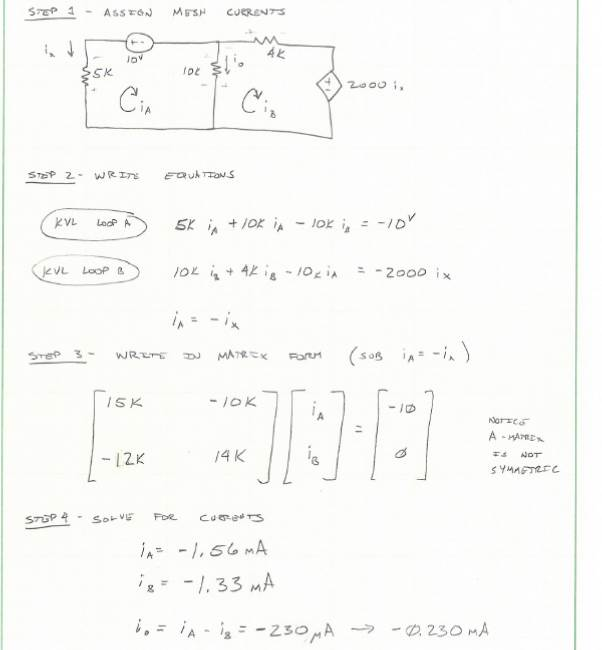
\includegraphics[width=0.8\textwidth]{Example6soln.jpg}
\end{figure}
}

\newpage
\clearpage
\pagebreak

\newpage
\clearpage
\pagebreak

\newpage
\clearpage
\pagebreak

\newpage
\clearpage
\pagebreak

\newpage
\clearpage
\pagebreak

\newpage
\clearpage
\pagebreak

\newpage
\clearpage
\pagebreak

\newpage
\clearpage
\pagebreak

\end{document}


% Equation Array Example Code
%\begin
%{eqnarray}
%P_R &=& i_R^2R \nonumber \\
%P_R &=& (100\ mA)^2 \times 100\ \Omega \nonumber \\
%P_R &=& (100 \times 10^{-3}\ A)^2 \times 100\ \Omega \\
%P_R &=& 10000 \times 10^{-6}\ A^2  \times 100\ \Omega \nonumber \\
%P_R &=& 1\ W  \nonumber
%\end{eqnarray}

% Figure Example Code
%\begin{figure} [h t b]
%\centering
%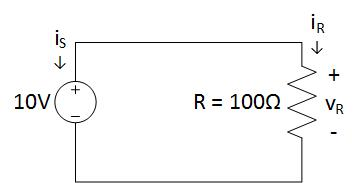
\includegraphics[width=0.5\textwidth]{OhmsLawExampleSolution.jpg}
%\caption{Ohm's Law example circuit}
%\label{fig: OhmsLawExampleSolution}
%\end{figure}

%Table Example Code
%\begin{table}[h]
%\centering
%\begin{tabular}{|l|c|c|}
%\hline
%Prefix & Abbreviation & Value \\
%\hline \hline
%Giga & $G$ & $10^9$ \\
%Mega & $M$ & $10^6$ \\
%Kilo & $k$ & $10^3$ \\
%\hline
%milli & $m$ & $10^{-3}$ \\
%micro & $\mu$ & $10^{-6}$ \\
%nano & $n$ & $10^{-9}$ \\
%pico & $p$ & $10^{-12}$ \\
%\hline
%\end{tabular}
%\caption{Engineering prefixes and values}
%\label{tab: Eng Prefixes}
%\end{table}
